% ---------
%  Compile with "pdflatex hw0".
% --------
%!TEX TS-program = pdflatex
%!TEX encoding = UTF-8 Unicode

\documentclass[11pt]{article}

\usepackage{graphicx, jeffe, handout}
\usepackage[utf8]{inputenc}		% Allow some non-ASCII Unicode in source
\usepackage[font=small,labelfont=bf]{caption}
\usepackage{fourier-orns}
\usepackage{amssymb}
\usepackage{changepage}
\usepackage[scaled=.7]{beramono}
\usepackage[labelfont=normalfont]{caption}
\usepackage{float}

%\Section{}

\pdfpagewidth 8.5in
\pdfpageheight 11in
\headheight 0pt
\headsep 0pt
\footskip .25in
\marginparwidth 0pt
\marginparsep 0pt
\oddsidemargin \dimexpr 1in -1in
\topmargin \dimexpr 1in -1in
\textwidth \dimexpr \pdfpagewidth -2\oddsidemargin -2in
\textheight \dimexpr \pdfpageheight -2\topmargin -2in
\setlength{\belowcaptionskip}{-10pt}


% =====================================================
\begin{document}

% ---------------------------------------------------------

\Class{ECE/CS 438}
\Semester{Fall 2017}
\Authors{2}
\AuthorOne{Rahul Sharma}{rsharm12}
\AuthorTwo{Srujun Thanmay Gupta}{sgupta80}
\HomeworkHeader{4}{}

\section*{CSMA Analysis}

\begin{enumerate}[a.]
% ----- PART A
\item The graph of channel utilization as a function of the increasing number of nodes appears to decrease as inversely proportional to a quadratic function. The reason for this is that with a larger number of nodes, the potential for collisions is significantly higher because more nodes can randomly choose values close enough to each other that they will attempt to transmit at the same time. Thus, the channel spends less and less time being utilized as the number of nodes increasing.

\begin{figure}[h]
\centering
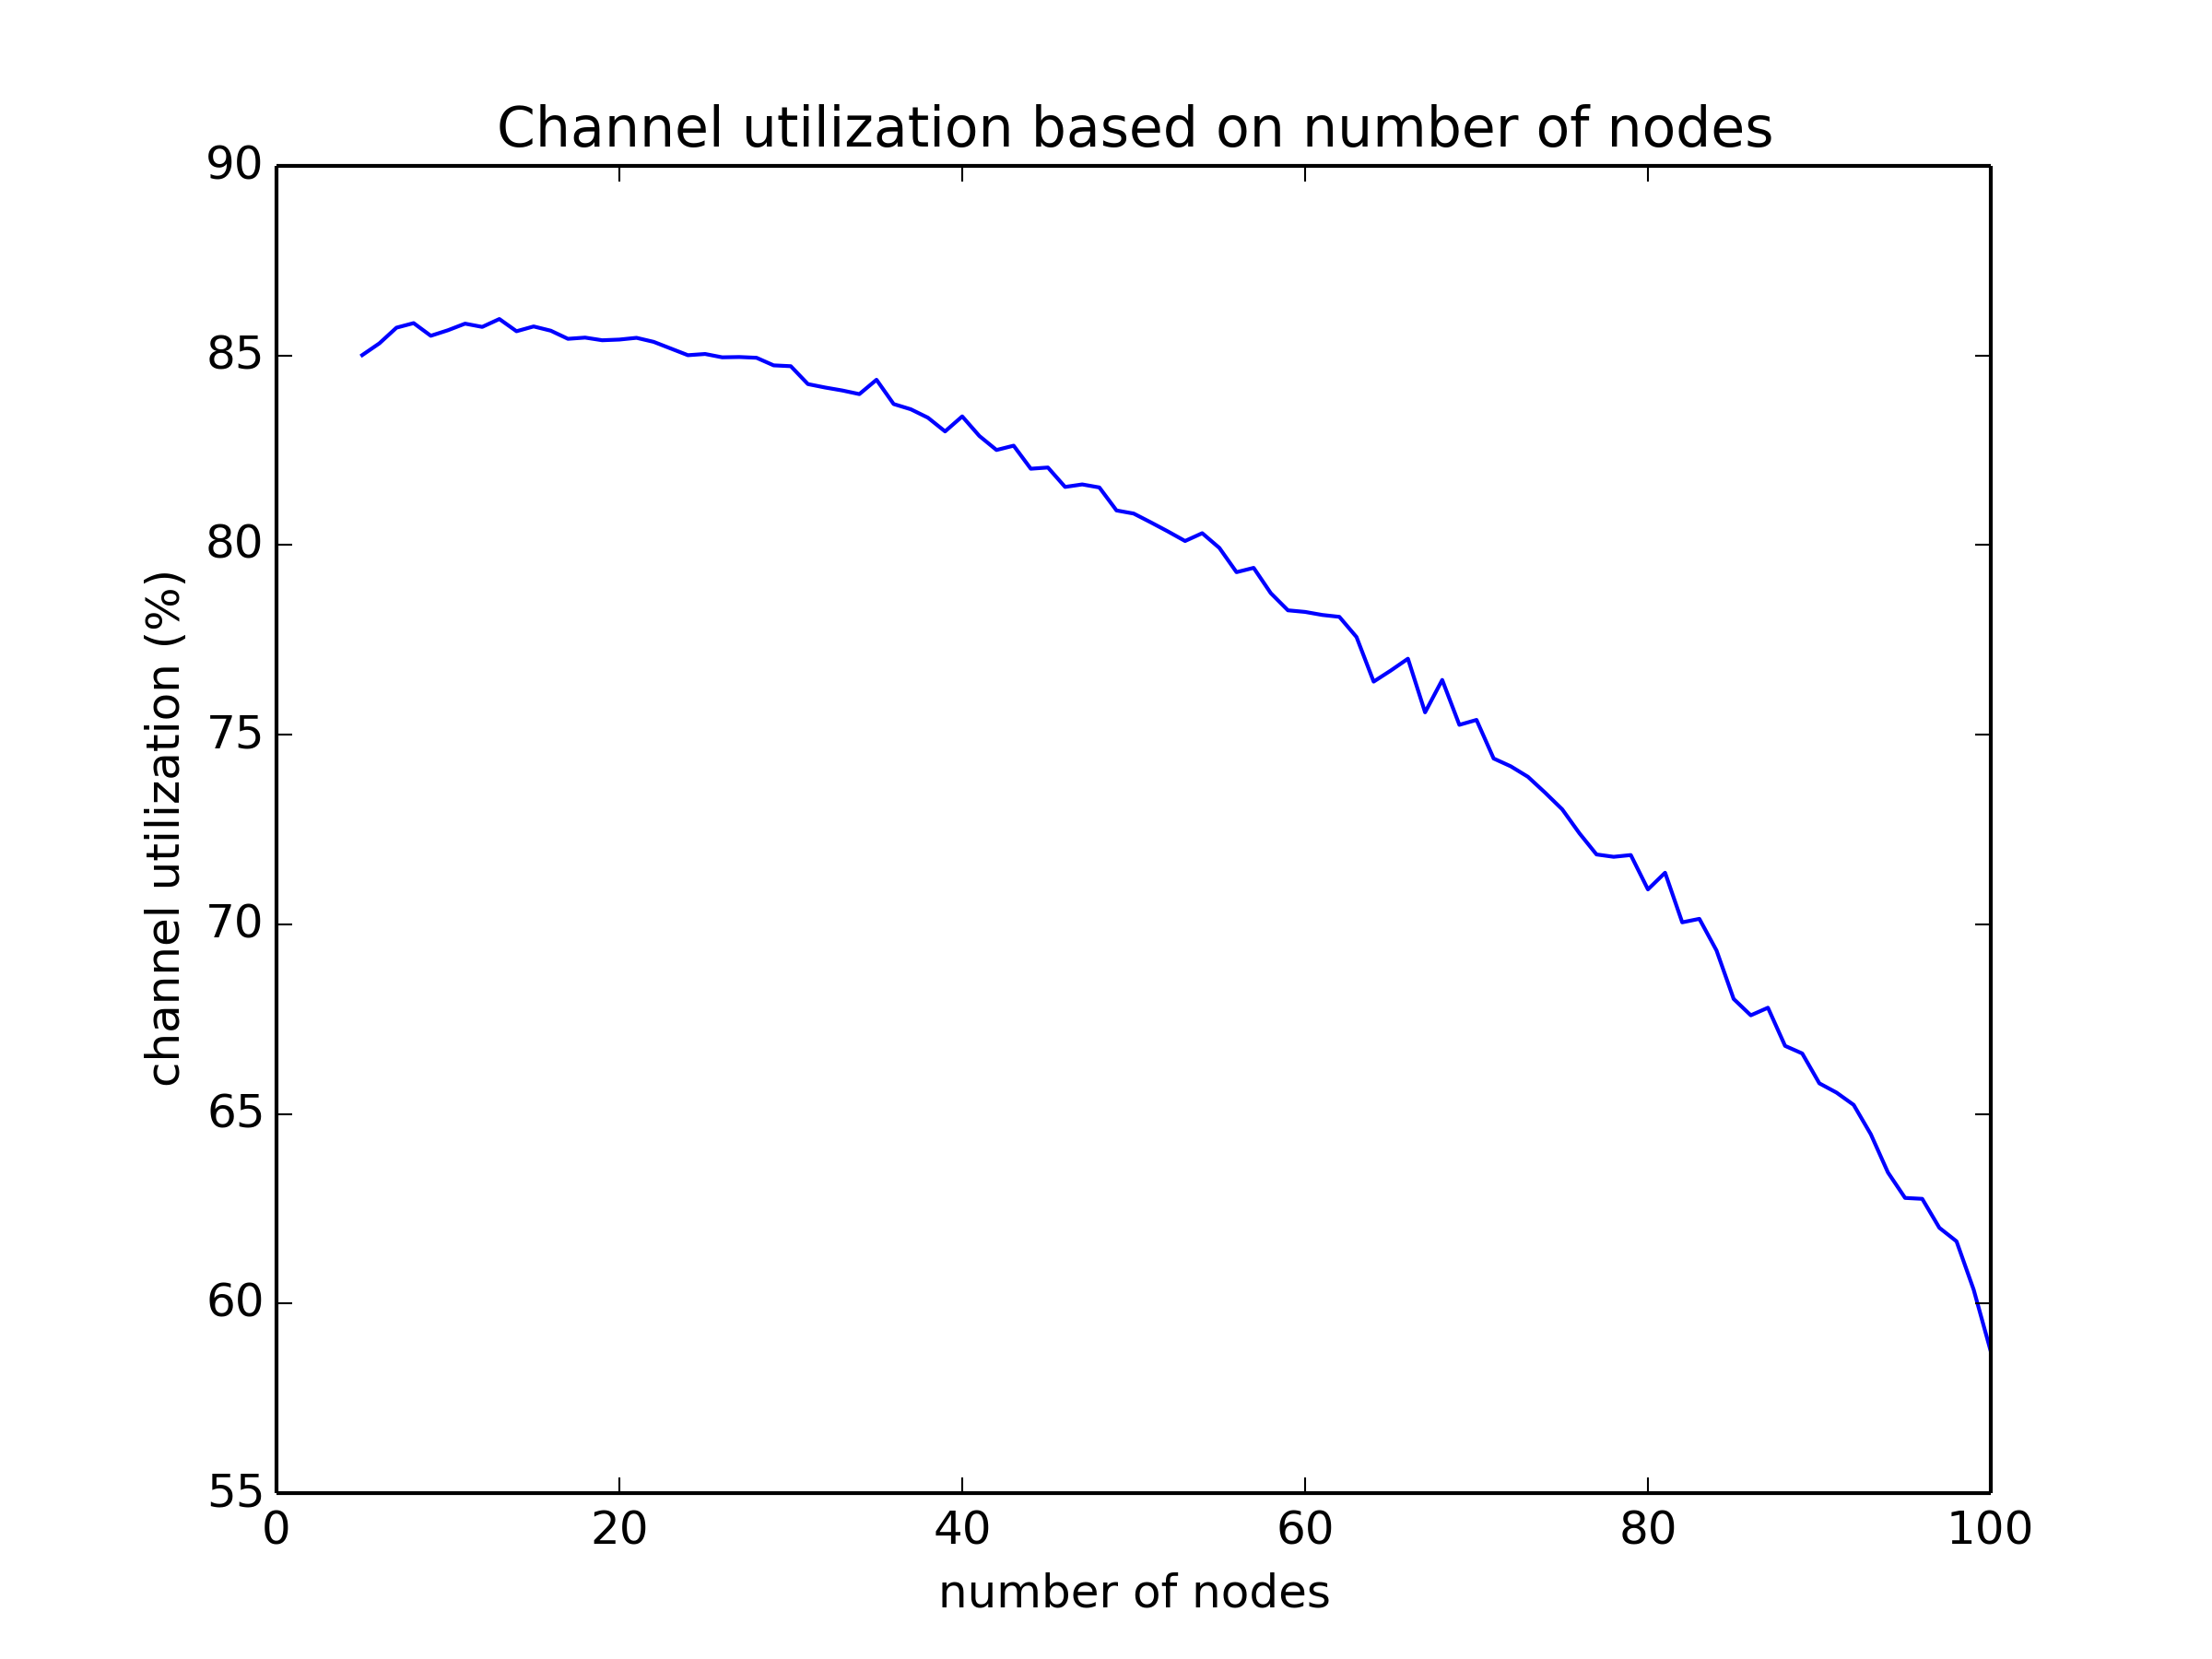
\includegraphics[width=.9\textwidth]{partA.png}
\caption{}
\end{figure}

\newpage

% ----- PART B
\vspace*{2mm}
\item Channel idle fraction doesn’t count the ticks where packets are actively colliding and so again similar to part a), as the number of nodes increases there is a significantly higher potential for packets to collide meaning the channel isn’t being utilized but it also is not idle. In the beginning however, there are fewer nodes in total so less nodes have the potential to transmit at all meaning the channel idle fraction is also higher.


\begin{figure}[H]
\centering
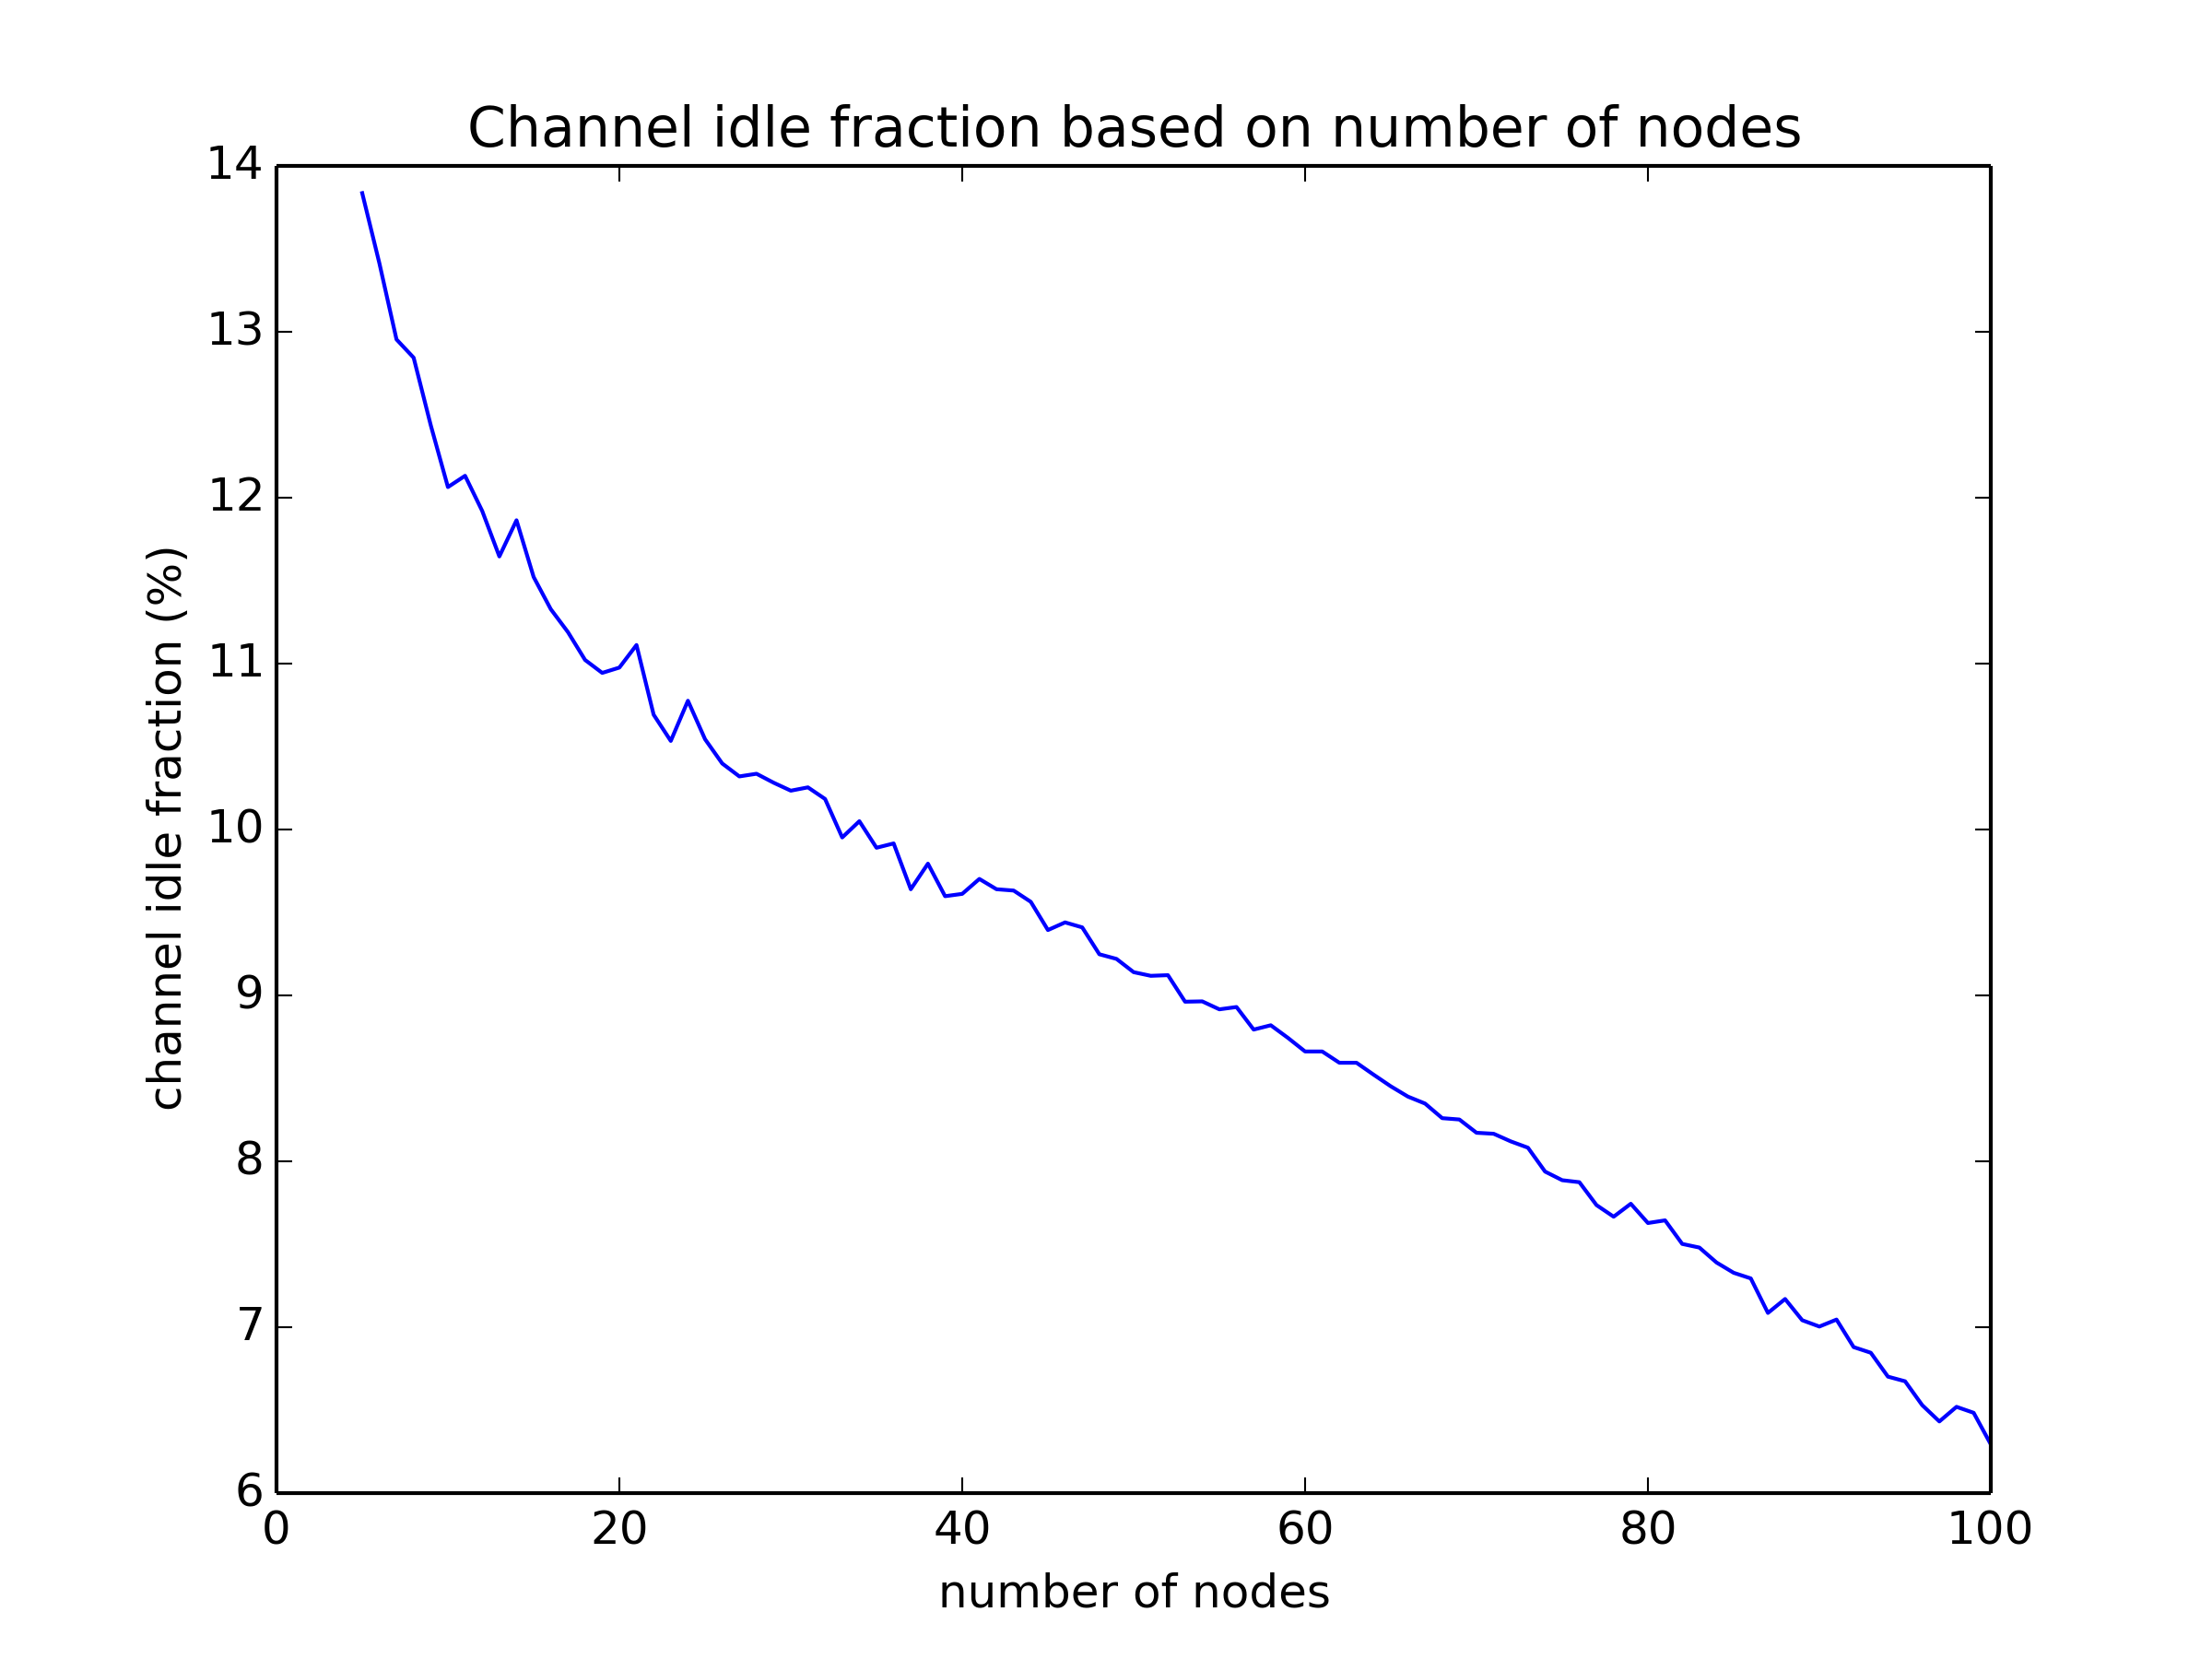
\includegraphics[width=.9\textwidth]{partB.png}
\caption{}
\end{figure}

\newpage

% ----- PART C
\vspace*{2mm}
\item As number of nodes increases, and the range of R still maximizes out at $128$ there are far more opportunities for collisions because the larger number of nodes can end up choosing the same number randomly. Note that the empirical results shown in the graph below only support this and the answers to both part a) and part b) where we relied on the notion that as number of nodes increases number of collisions increases.

\begin{figure}[H]
\centering
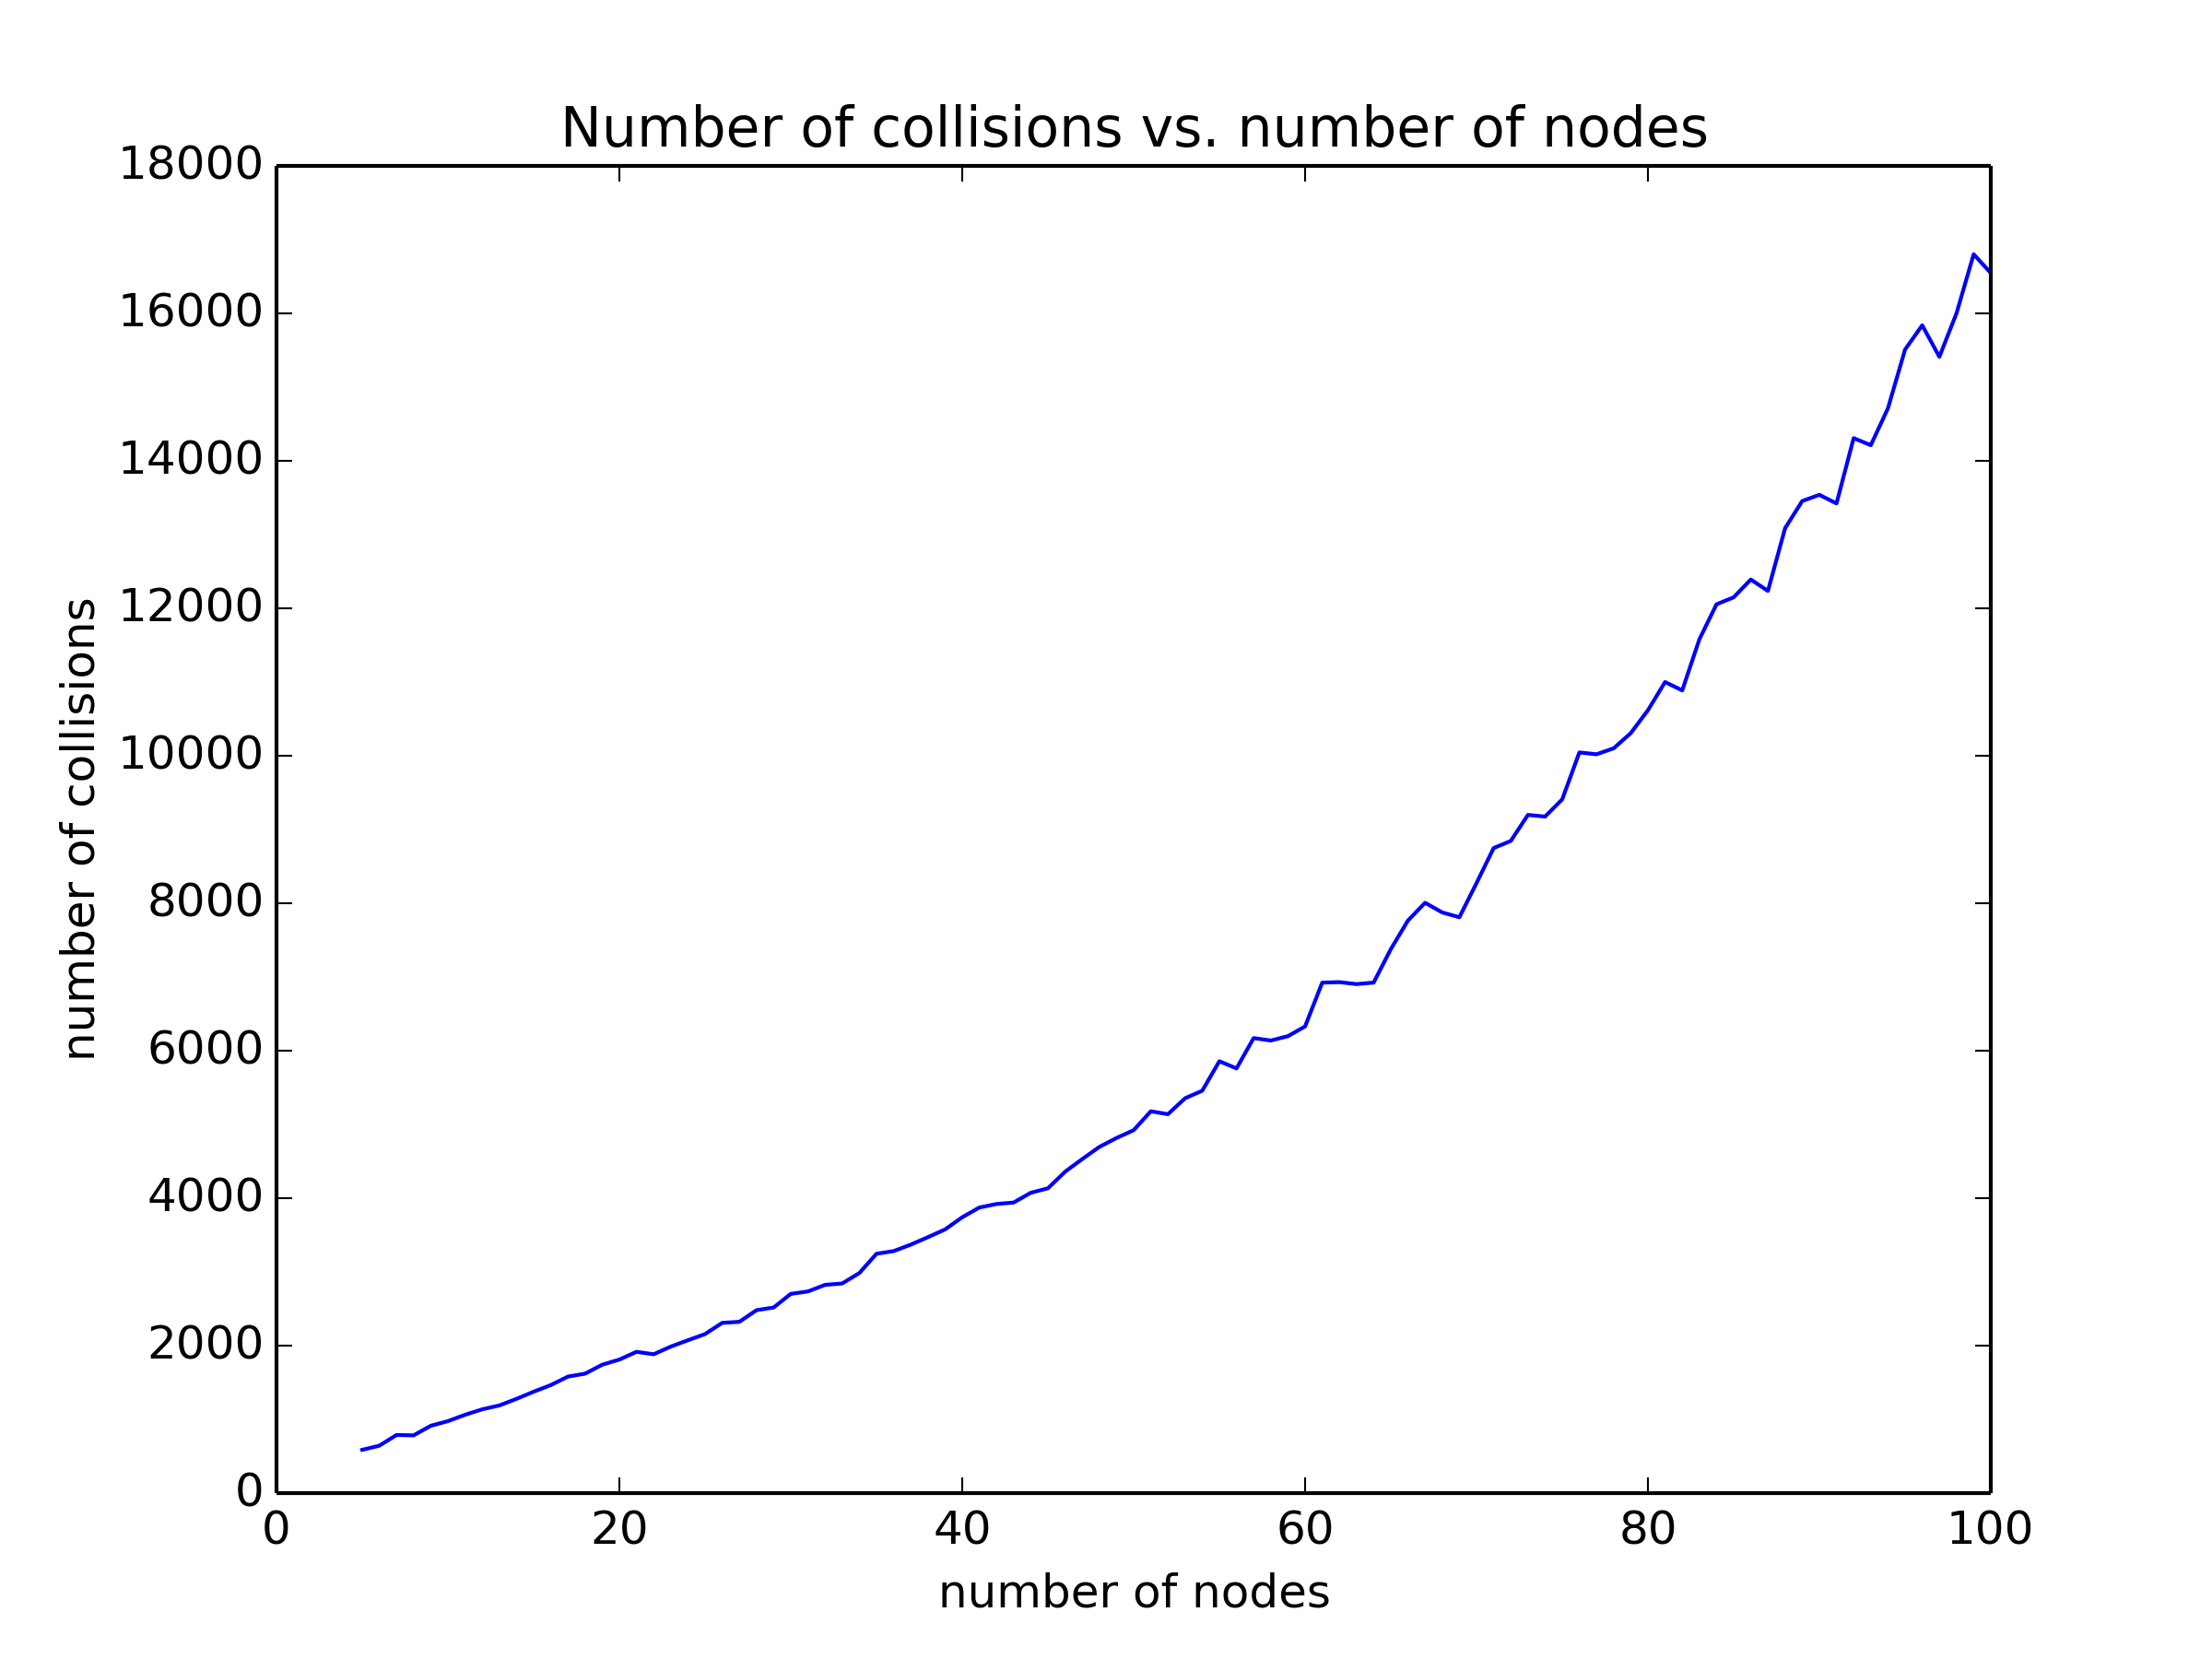
\includegraphics[width=.9\textwidth]{partC.png}
\caption{}
\end{figure}

\newpage

% ----- PART D
\vspace*{2mm}
\item In the results shown in figure $4$, we can see that the increase in the number of nodes first increases the utilization as more nodes are able to take advantage of the full backoff range, but after this peak the number of collisions increases and channel utilization drops off as the nodes spend less time transmitting.

\begin{figure}[H]
\centering
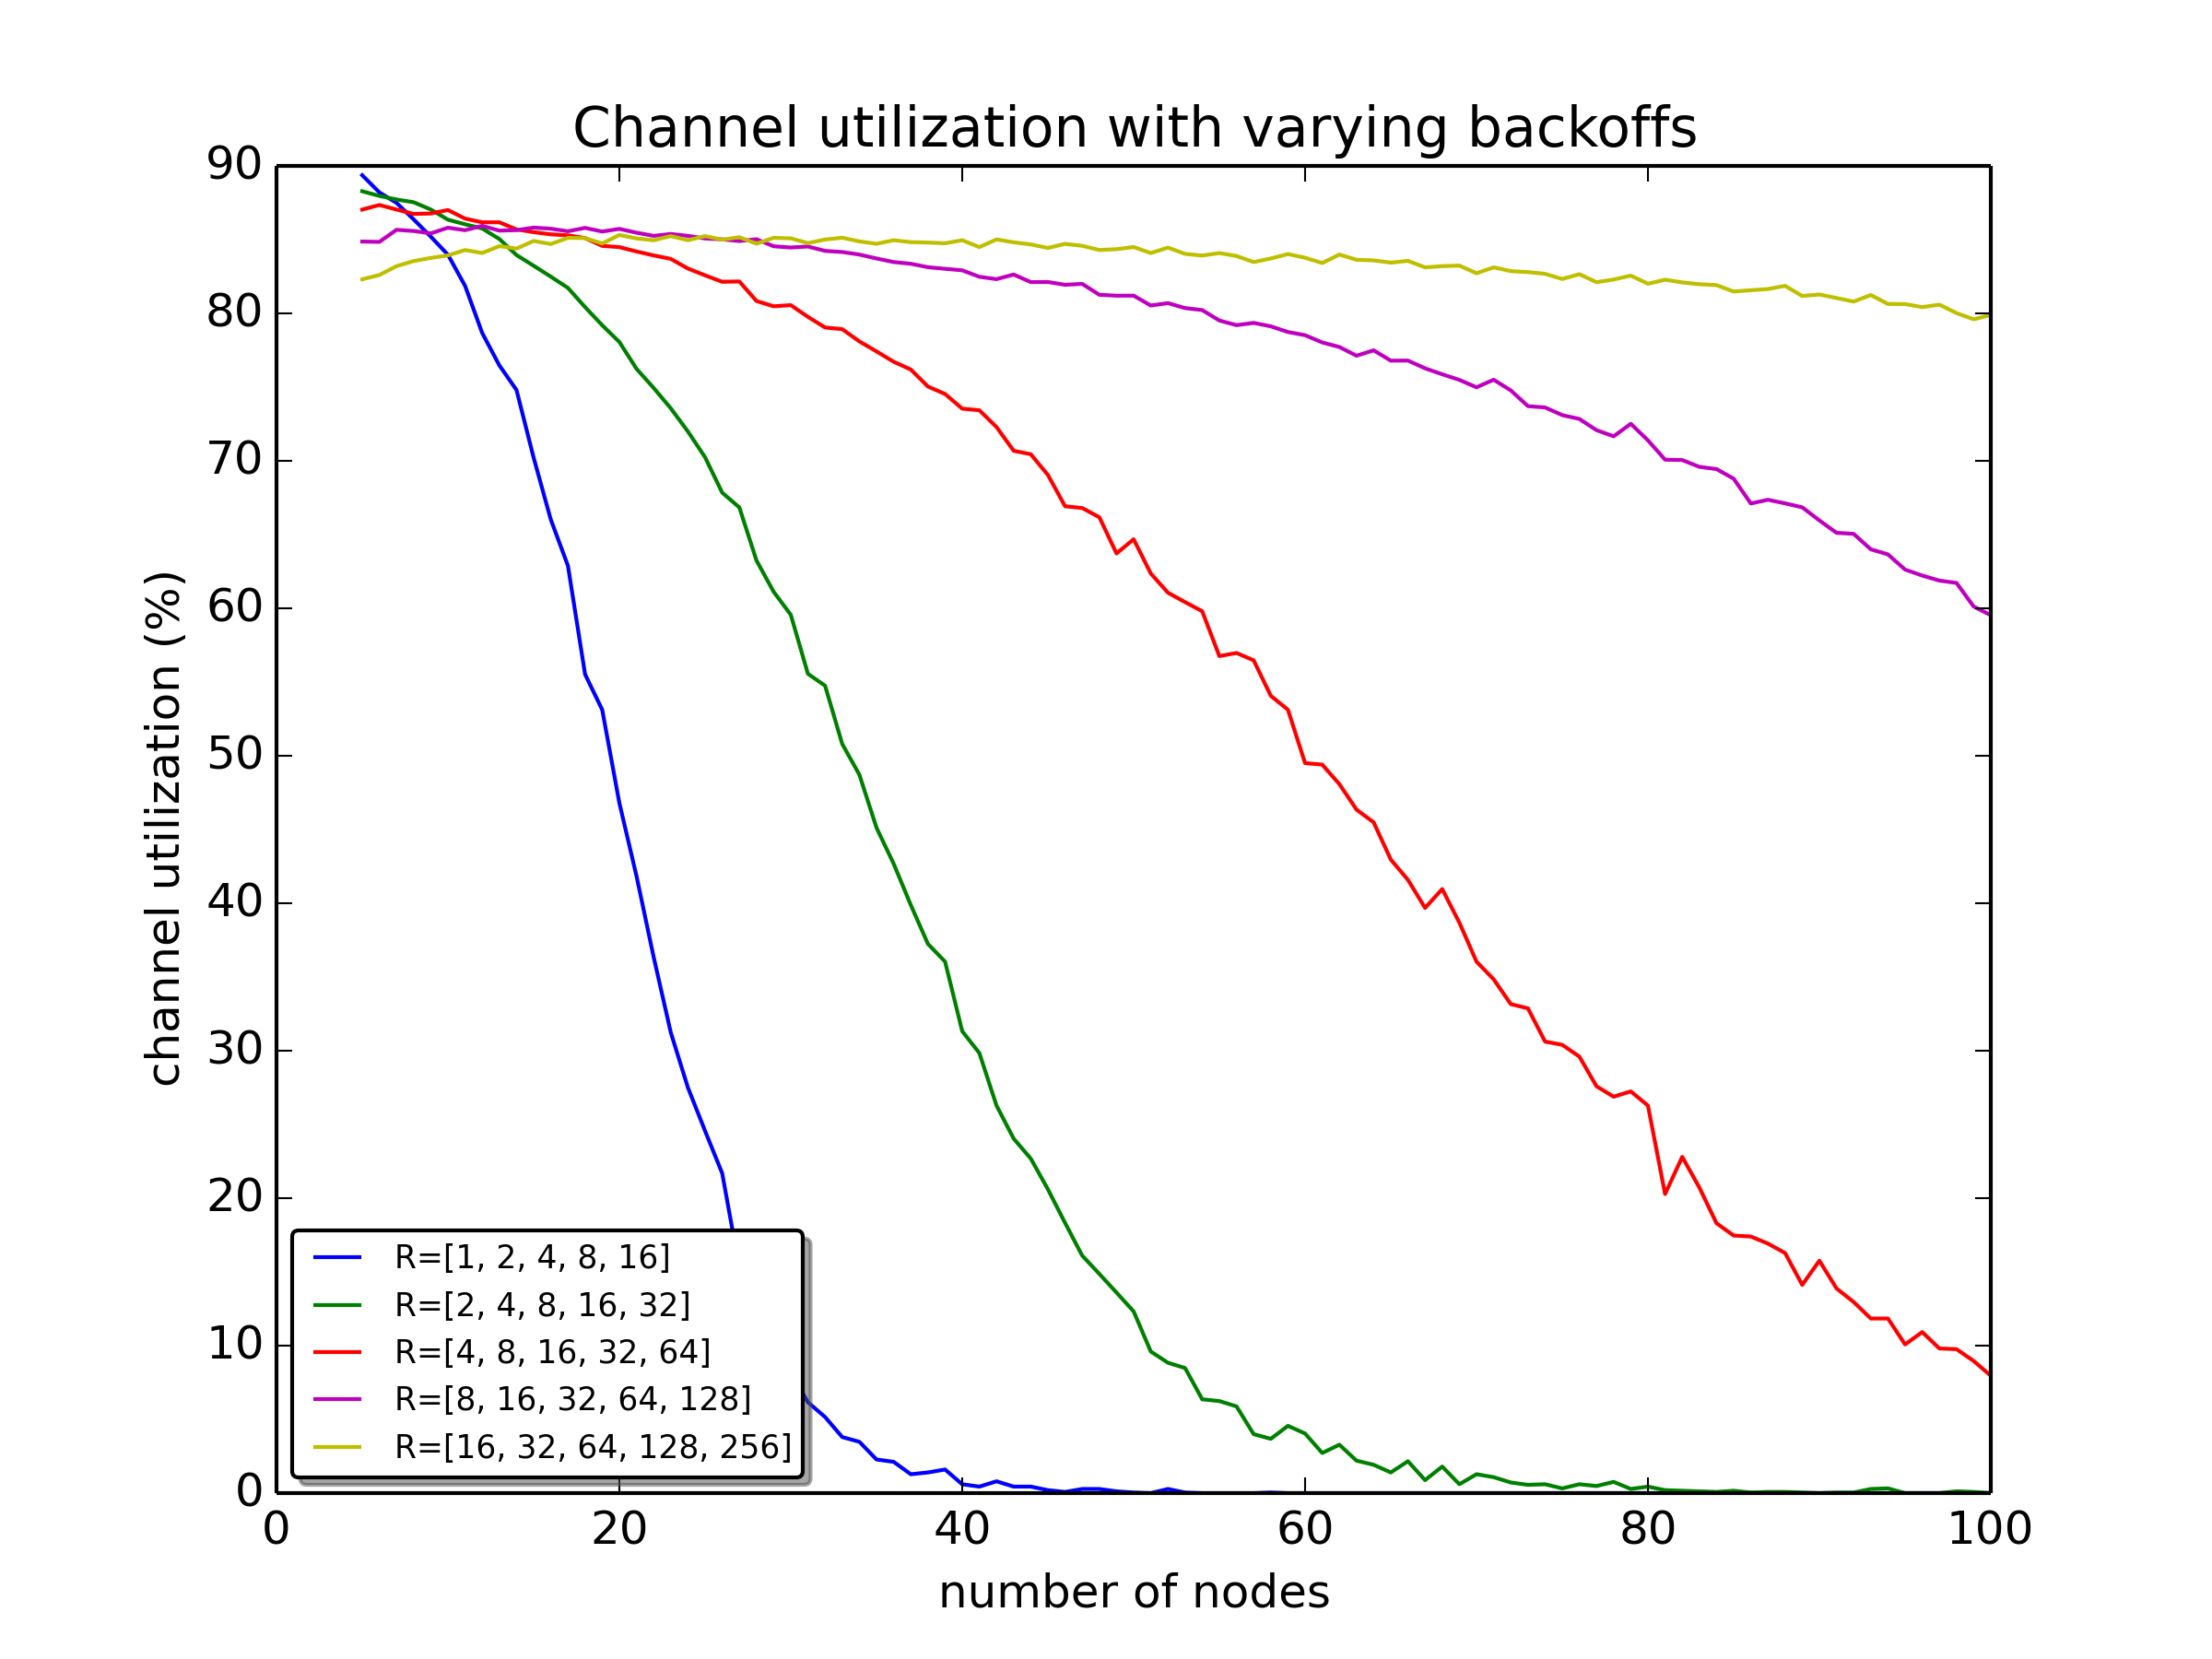
\includegraphics[width=.9\textwidth]{partD.png}
\caption{}
\end{figure}

\newpage

% ----- PART E
\vspace*{2mm}
\item We can still see the quadratic dropoff in the lines for each L because as the number of nodes increases the number of collisions increases as seen in figure 3 above. 

\begin{figure}[H]
\centering
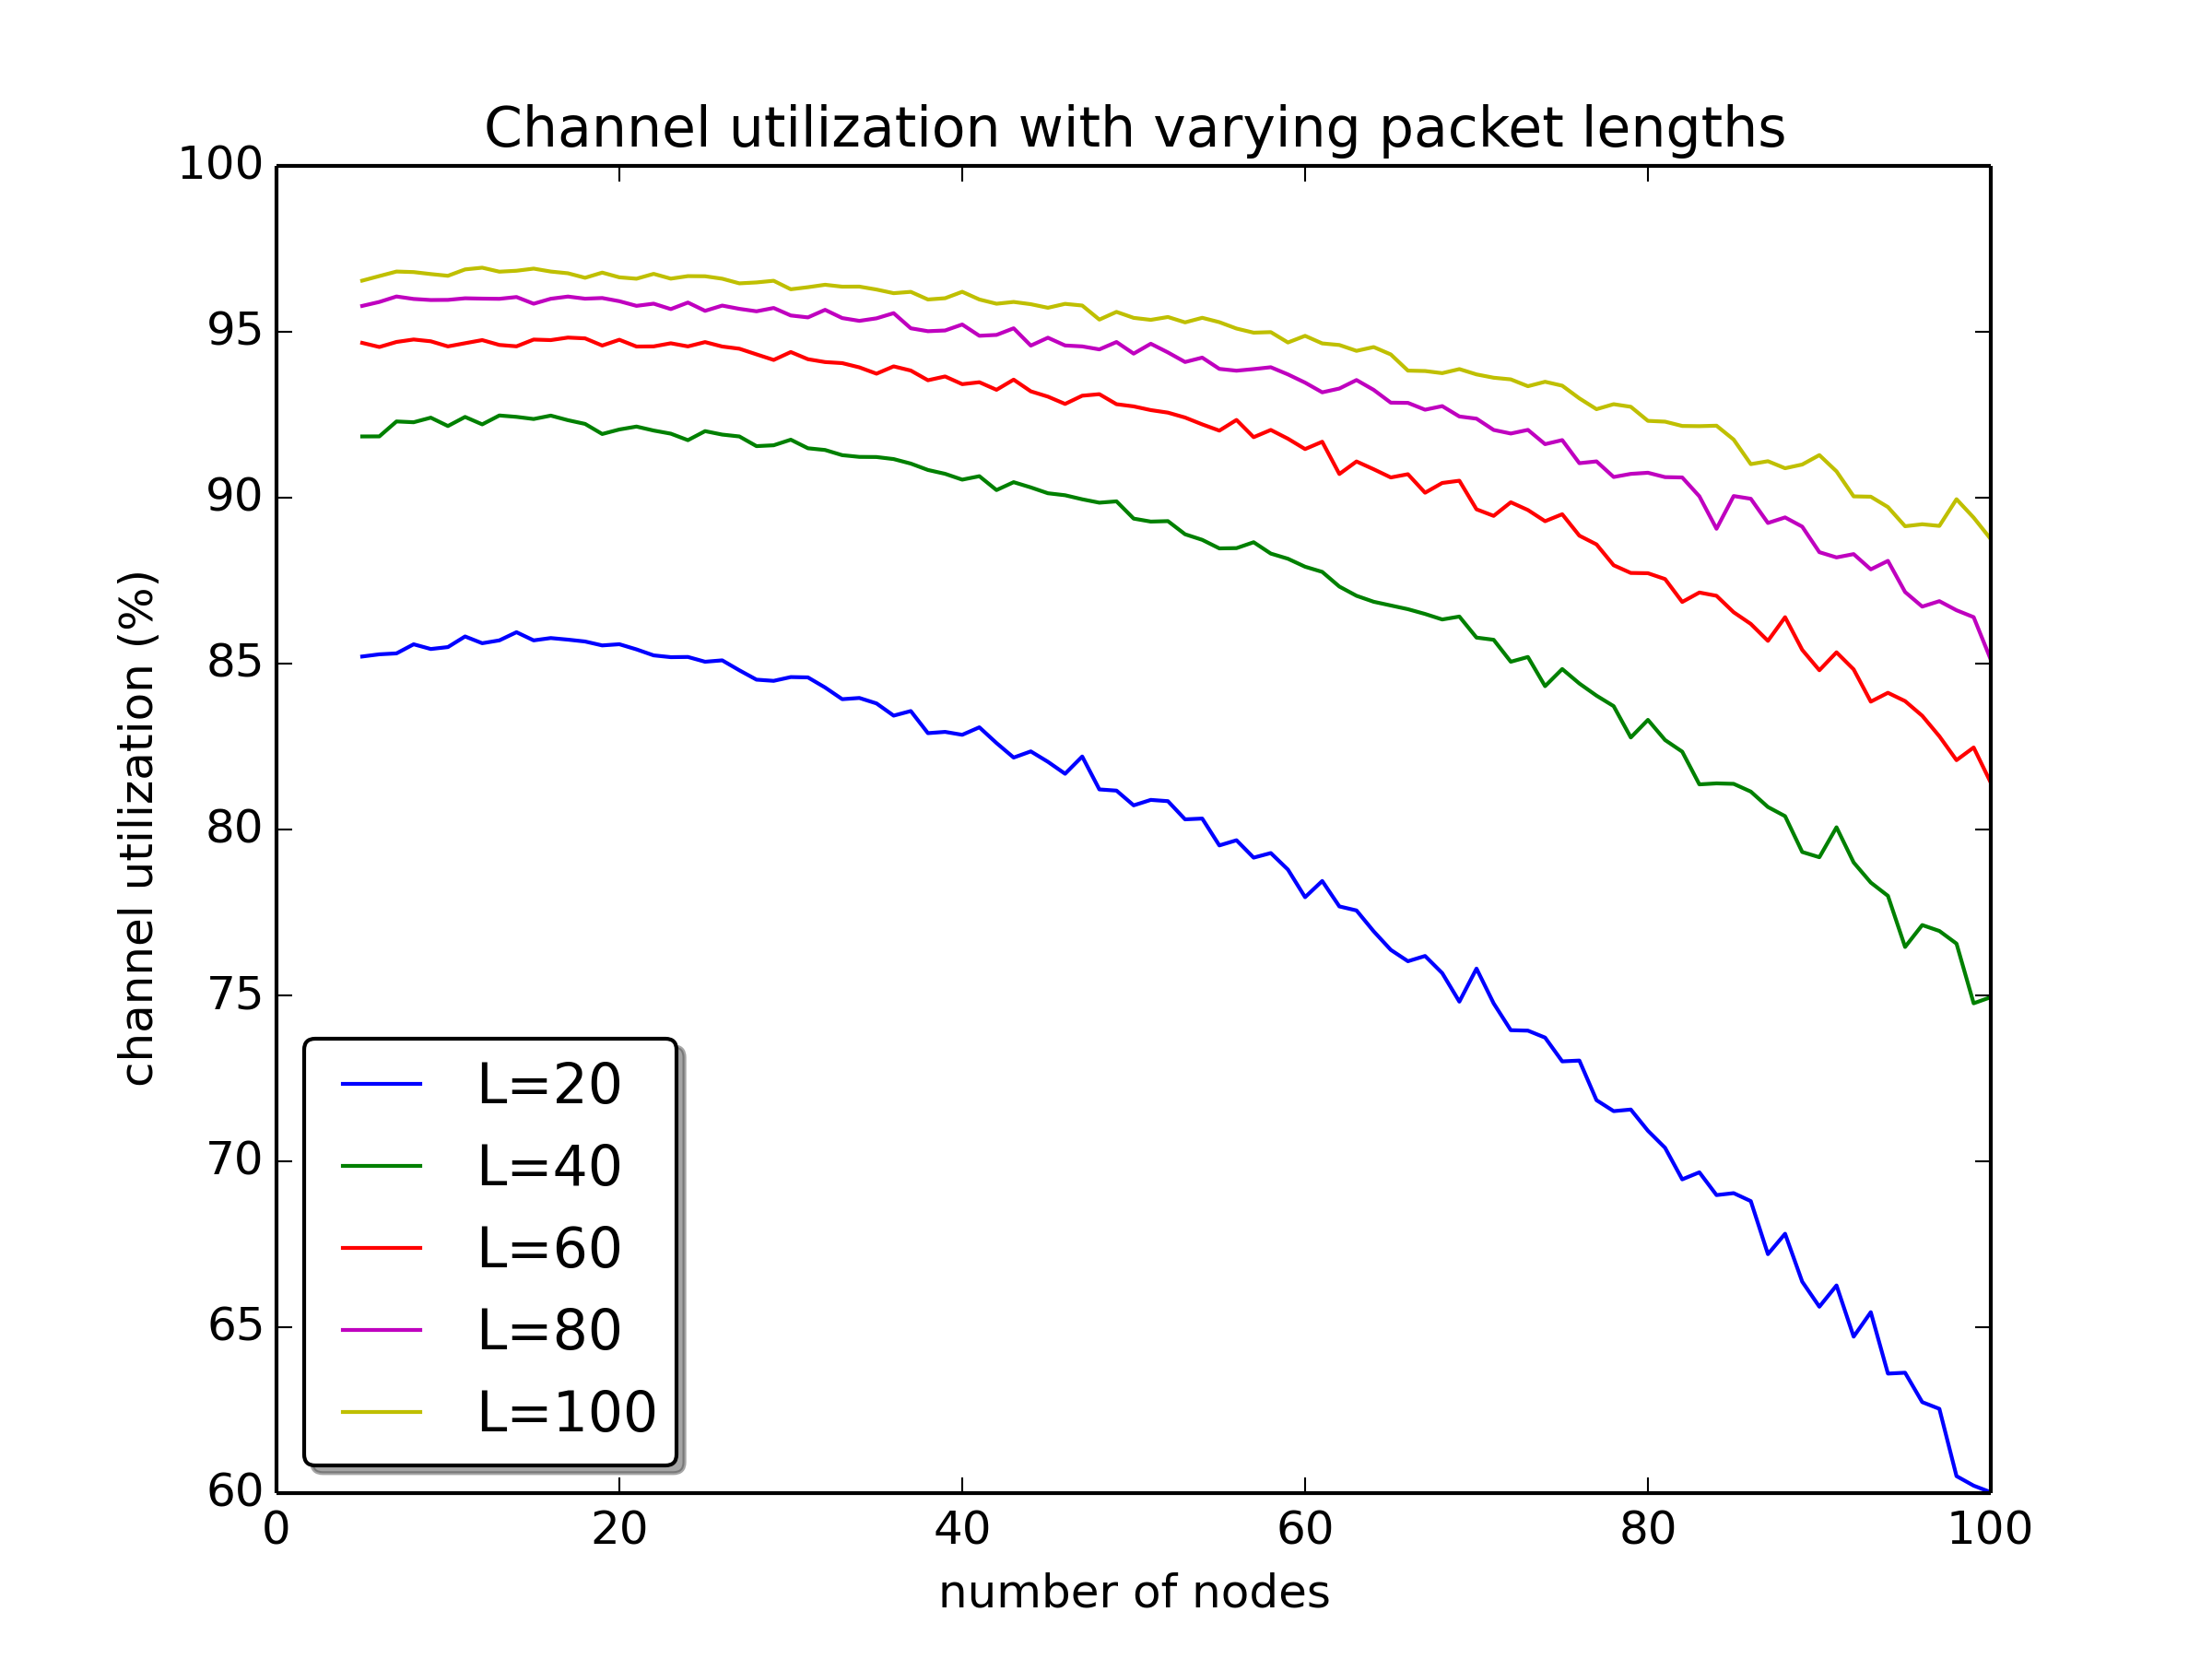
\includegraphics[width=.9\textwidth]{partE.png}
\caption{}
\end{figure}

% ------ PART F
\vspace*{2mm}
\item As the backoff ranges for R increase, there are more random numbers for nodes to choose from thus decreasing the total number of collisions. For the lowest backoff range (starting from R=$1$), we can see that the channel utilization effectively goes to $0$ because the number of nodes far exceeds the range of the backoff and so for a successful transmission to occur one node will have to pick a value while all the others choose a different value. Similarly, in figure 5 we can see the effect of packet length on channel utilization. Here we can see that as L increases, the channel utilization increases as well because the channel spends a longer time transmitting a packet thus increasing the overall channel utilization. In general, as N increases channel utilization decreases because simply put, there are more nodes attempting to transmit and thus more opportunity for conflict. This observation is evident in every graph.


\end{enumerate}


\end{document}
